% FastPose-ViT-MO: draft of the follow-up paper on multi-object 6D pose estimation on BOP.
% Structure and style follow docs/PAPER_FEAT.md (same skeleton as the WACV 2026 paper);
% numbers come from docs/BOP.md and TASKS.md §9. Sections whose results are still running
% are marked with \pending{...}. Compile with pdflatex + bibtex (Overleaf: default settings).
%
% Template: with the official WACV/CVF style files (wacv.sty and ieeenat_fullname.bst or
% ieee_fullname.bst) uploaded next to this file, the draft compiles in the WACV review format;
% without them it falls back to a plain two-column article so that it compiles anywhere.
%
% Two documents share preamble.tex and references.bib: main.tex (the paper) and
% supplementary.tex (the supplementary material, a separate PDF; the paper refers to its sections
% as "Supp. Sec. S1-S8").
%
% Status (2026-11-14):
%   done     LM-O, YCB-V, all ablations except bbox jitter 5 / 15 / 30 % (seed a), augmentation
%            study, deployment and latency, own detector, figures (paper/figures, made by
%            vis/paper_*.py), verified leaderboard and bibliography, supplementary split.
%   running  T-LESS (tless-m10-tok4x{,2}-002, epochs 128 / 104 of 150); bbox jitter
%            lmo-m10-bbox{5,52,15,30}-003 (relaunched after a node failure).
%   open     positioning vs PViT-6D / PoseDETR (to agree with the supervisor), venue and page
%            limit, authors, Jetson latency. Search for \pending and \todo.
% Shared preamble of main.tex and supplementary.tex (same packages, macros and notation).
\documentclass[10pt,twocolumn,letterpaper]{article}

\IfFileExists{wacv.sty}{%
  \usepackage[review]{wacv}
  \def\paperID{*****}
  \def\confName{WACV}
  \def\confYear{2027}
}{%
  \usepackage[margin=0.75in,columnsep=0.25in]{geometry}
  \usepackage{times}
}

\usepackage{amsmath,amssymb,bm}
\usepackage{graphicx}
\usepackage{booktabs}
\usepackage{multirow}
\usepackage{xcolor}
\usepackage[hidelinks]{hyperref}
\usepackage[capitalize]{cleveref}

% Draft helpers: \pending for results still running, \todo for things to write or check.
\newcommand{\pending}[1]{\textcolor{orange}{[\textbf{Pending:} #1]}}
\newcommand{\todo}[1]{\textcolor{red}{[\textbf{TODO:} #1]}}
\newcommand{\figplaceholder}[2]{\fbox{\parbox[c][#1][c]{0.95\linewidth}{\centering\small #2}}}

% Notation (\eg is defined by the WACV style; fallback otherwise)
\providecommand{\eg}{e.g.\@\xspace}
\usepackage{xspace}
\newcommand{\R}{\mathbf{R}}
\newcommand{\T}{\mathbf{T}}
\newcommand{\K}{\mathbf{K}}
\newcommand{\U}{\mathbf{U}}
\newcommand{\ours}{FastPose-ViT-MO}


\title{\ours: Real-Time Multi-Object 6D Pose Estimation by Direct Regression}

\author{%
  Pablo Sarro\\
  EPFL\\
  {\tt\small \todo{email; co-authors and affiliations (e.g.\ supervisors) to agree}}
}

\begin{document}
\maketitle

\begin{abstract}
Estimating the 6D pose of every object in an RGB image is a core problem for robotic
manipulation and augmented reality. The strongest RGB methods on the BOP benchmark predict 2D--3D
correspondences and solve for the pose with PnP, often train one network per object, and many add
an iterative render-and-compare refinement, which makes them slow and hard to deploy on embedded
hardware. We present \ours{}, a multi-object extension of FastPose-ViT that regresses the full 6D
pose of every detected object directly from its image crop, with one Vision Transformer shared by
all objects of a dataset and no PnP or refinement. A per-object class token conditions the shared
network on the object identity, a camera- and object-size-independent translation target makes
the formulation valid across objects and cameras, and a symmetry-aware rotation loss with
translation offsets handles symmetric objects. Trained on synthetic (PBR) images only, \ours{}
reaches an average recall of 0.668 on LM-O and 0.702 on YCB-V with the standard BOP detections,
the best result among direct-regression methods and within 0.03--0.06 of the best PBR-only RGB
methods. Exported to TensorRT in FP16 without any loss in accuracy, the pose stage processes 8
objects in 14.2\,ms on an NVIDIA A100; with our own multi-class detector, the full pipeline runs
at 57 frames per second for 8 objects.
\todo{Update with T-LESS and the final latency numbers; check the word count (WACV: ~200 words).}
\end{abstract}

\section{Introduction}
\label{sec:intro}

\begin{figure*}[t]
  \centering
  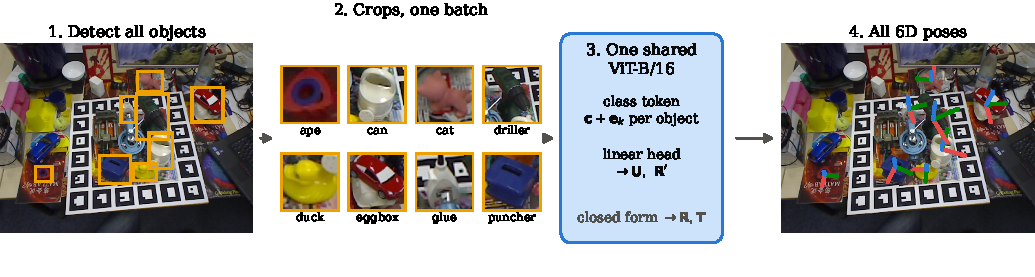
\includegraphics[width=\linewidth]{figures/teaser.pdf}
  \caption{\textbf{Overview of \ours.} (1) A detector finds every object of the dataset in the
  image; (2) each detection is cropped and all crops are processed in one batch by a single
  Vision Transformer, conditioned on the object identity by a per-object class token; (3) the
  regressed normalized translation and apparent rotation are converted in closed form into the
  full-frame pose. Real LM-O test image with the default detections and our predictions.
  \todo{First version made from real data; redraw as a clean diagram if preferred, and add the
  latency inset (\cref{fig:latency}).}}
  \label{fig:teaser}
\end{figure*}

Estimating the 3D rotation and translation (6D pose) of known objects from a single RGB image is a
key component of robotic grasping, augmented reality and autonomous inspection. The BOP
benchmark~\cite{hodan2018bop,hodan2020bop} has become the standard way to compare such methods:
it evaluates the poses of all annotated objects in real test images with the average recall (AR)
of three pose-error functions, and it encourages training on photorealistic synthetic (PBR)
images only~\cite{denninger2019blenderproc}.

The top RGB methods on BOP are \emph{hybrid}: a network predicts dense 2D--3D correspondences and
a PnP solver, usually inside RANSAC, recovers the pose~\cite{su2022zebrapose,hodan2020epos,li2019cdpn}.
Several of them train one network per object~\cite{wang2021gdrnet,liu2022gdrnpp}, and
render-and-compare methods add an iterative refinement stage~\cite{labbe2020cosypose,haugaard2022surfemb}.
These designs are accurate but expensive: the reported times on BOP range from 0.2\,s to
several seconds per image on desktop GPUs, and the number of networks grows with the number of
objects. \emph{Direct-regression} methods predict the pose with a single forward pass and are
much cheaper; recent ones close much of the gap with a single model for all objects, \eg
PViT-6D~\cite{stapf2023pvit6d} with a multi-scale ViT and PoseDETR as a single-stage detector.

FastPose-ViT~\cite{ancey2026fastposevit} showed that a Vision Transformer that directly regresses
a reformulated pose target from an object crop can be competitive with PnP-based methods for
spacecraft pose estimation, and can run in real time on an embedded Jetson device. It handles one
object, seen by one camera. In this work we ask whether the same direct-regression approach
scales to the multi-object, multi-camera setting of BOP, with one network for all objects and
synthetic training data only. To this end, we make the following contributions:
\begin{itemize}
  \item A \textbf{multi-object extension of FastPose-ViT} that keeps its simplicity: one plain
        ViT with a single linear layer, shared by all objects of a dataset and conditioned on the
        object identity by a learned per-object class token. It adds fewer than 0.05\,M
        parameters, batches the crops of different objects together, and matches eight
        single-object models trained with the same total compute.
  \item The \textbf{geometric targets for many objects and cameras}: per-image intrinsics and a
        size-invariant depth target (as in~\cite{stapf2023pvit6d}) in place of the original
        image-size-based one, which fails across objects of different sizes (+0.04 AR on LM-O),
        together with the apparent rotation, which we show remains essential on BOP (+0.11 AR).
  \item A \textbf{symmetry-aware rotation loss with translation offsets}, which takes the
        minimum over the symmetric poses of an object, including symmetries that also shift the
        object, and stays valid on the apparent-rotation targets.
  \item A \textbf{deployment study} on BOP: batched TensorRT FP16 inference with no loss in AR,
        latency as a function of the number of objects, and a multi-class LW-DETR
        detector~\cite{chen2024lwdetr} that brings the full pipeline to 55 frames per second for
        8 objects on an A100.
\end{itemize}
Trained on PBR images only, \ours{} reaches an AR of 0.668 on LM-O~\cite{brachmann2014lmo} and
0.702 on YCB-V~\cite{xiang2018posecnn} with the standard BOP detections. On YCB-V, this is the
best result among PBR-only RGB methods with one model for all objects, behind only two methods
that train one network per object; on LM-O, it is within 0.07 AR of the best PBR-only RGB methods.
\todo{Positioning to agree with the supervisor: PViT-6D (0.740) and PoseDETR (0.695) are more
accurate on LM-O.}
\pending{T-LESS result (jobs running), to add to this paragraph.}

\section{Related Work}
\label{sec:related}

\paragraph{Correspondence-based 6D pose estimation.}
Most leading RGB methods on BOP predict 2D--3D correspondences and solve for the pose with
PnP. EPOS~\cite{hodan2020epos} predicts dense surface fragments, CDPN~\cite{li2019cdpn}
disentangles rotation (from correspondences) and translation (regressed),
ZebraPose~\cite{su2022zebrapose} encodes surface points with hierarchical binary codes, and
GDR-Net / GDRNPP~\cite{wang2021gdrnet,liu2022gdrnpp} learn the PnP step from geometric
intermediate maps. These methods top the PBR-only RGB leaderboards, but most of them train one
network per object, and their inference includes PnP-RANSAC or several stages. In contrast, we
regress the pose directly with one network shared by all objects.

\paragraph{Render-and-compare and refinement.}
CosyPose~\cite{labbe2020cosypose}, SurfEmb~\cite{haugaard2022surfemb} and
MegaPose~\cite{labbe2022megapose} refine an initial estimate by rendering the object model and
comparing it with the image, iteratively. Refinement improves accuracy, but it multiplies the
inference time (up to seconds per image) and requires a renderer at test time. We use no
refinement; our estimates could serve as initialization for such a stage.

\paragraph{Direct regression and Transformers.}
Direct methods regress the rotation and translation from image features in a single forward
pass. The choice of the targets matters: continuous rotation representations~\cite{zhou2019continuity},
allocentric (apparent) rotations~\cite{kundu20183drcnn}, and scale-invariant translation
targets~\cite{li2019cdpn,wang2021gdrnet}. PViT-6D~\cite{stapf2023pvit6d} regresses the pose
of each detection with a multi-scale ViT (MViTv2) shared by all objects: separate rotation and
translation tokens, initialized with a learned embedding of the detected class, feed two MLP
heads; it introduces a size-invariant depth target that normalizes the depth by the object
diameter, which we also use (\cref{sec:method:translation}), and reaches 0.73--0.74 AR on LM-O
with PBR training. PoseDETR and RACE-6D (BOP leaderboard submissions) predict instances and poses
in a single stage at about 12\,ms per image. FastPose-ViT~\cite{ancey2026fastposevit} regresses normalized
translation targets and the apparent rotation from object crops with a ViT and a single linear
head, and runs in real time on a Jetson Orin Nano, but for one object and one camera only. We
extend it to many objects and cameras with a plain ViT and a single linear layer, and evaluate it
on BOP. \todo{Sharpen the difference with PViT-6D (plain ViT-B and one linear layer vs MViTv2 with
pose tokens and MLP heads; symmetric loss with offsets; deployment study) and cite PoseDETR /
RACE-6D papers when available.}

\paragraph{Fast object detectors.}
Two-stage pose pipelines depend on a 2D detector. The BOP default detections for the 2023
challenge come from the GDRNPP detector~\cite{liu2022gdrnpp}, which takes about 80\,ms per image.
Real-time DETR variants such as LW-DETR~\cite{chen2024lwdetr} make the detector much cheaper; we
train a multi-class LW-DETR on the same PBR images to obtain a fully real-time pipeline.

\section{Methodology}
\label{sec:method}

Given an RGB image with known camera intrinsics $\K$ and a set of known objects, our goal is to
predict, for every visible object instance, its rotation $\R \in SO(3)$ and translation
$\T \in \mathbb{R}^3$ from the model frame to the camera frame. As in
FastPose-ViT~\cite{ancey2026fastposevit}, a 2D detector first provides a bounding box and an
object label for each instance; the pose network then works on the image crop around each box.
\Cref{sec:method:recap} summarizes the original formulation, and
\cref{sec:method:translation,sec:method:conditioning,sec:method:symmetry,sec:method:training}
describe what changes for multiple objects and cameras.

\subsection{Recap: FastPose-ViT}
\label{sec:method:recap}
The crop is resized to the input size of a ViT-B/16~\cite{dosovitskiy2021vit} pretrained with
SWAG~\cite{singh2022swag}, and a single linear layer on the [CLS] token outputs nine values: three
normalized translation parameters $\U = (U_x, U_y, U_z)$ and a 6D rotation
representation~\cite{zhou2019continuity}, converted into a rotation matrix by Gram--Schmidt
orthonormalization. The network does not regress the absolute rotation $\R$, which depends on
where the object lies in the image, but the \emph{apparent rotation}
$\R' = \Delta\R\,\R$, where $\Delta\R$ rotates the viewing ray of the object centre
$\hat{\T} = \T / \|\T\|$ onto the optical axis $\mathbf{e}_z$. $\Delta\R$ has axis
$\mathbf{u} = \hat{\T} \times \mathbf{e}_z$ and angle $\theta = \arccos(\hat{\T}^\top
\mathbf{e}_z)$, and is computed in closed form with Rodrigues' formula; at inference,
$\R = \Delta\R^\top \R'$ once $\T$ is known. We keep the apparent rotation, the 6D
representation and the relative Frobenius rotation loss of~\cite{ancey2026fastposevit} unchanged,
and refer to it for their derivation.

\subsection{Camera- and size-independent translation}
\label{sec:method:translation}
Let $(b_x, b_y)$, $w$ and $h$ be the centre, width and height of the bounding box in pixels, and
$f_x, f_y, c_x, c_y$ the intrinsics of the image, which on BOP change from one image (and dataset)
to the next. The lateral targets measure where the projected object centre lies relative to the
box, in box units, as the scale-invariant translation of CDPN~\cite{li2019cdpn}:
\begin{equation}
  U_x = \frac{f_x \, t_x / t_z + c_x - b_x}{w}, \qquad
  U_y = \frac{f_y \, t_y / t_z + c_y - b_y}{h}.
  \label{eq:uxy}
\end{equation}
For the depth, the original formulation used a crop-depth proxy proportional to $t_z$ times the
box size divided by the image size. This proxy is well scaled for a single object and a single
camera, but on BOP it depends on the object size and the focal length: on LM-O it ranges from
about 50 to 300 (with $t_z$ in mm), while $U_x$ and $U_y$ stay within about $\pm 0.5$, so a
relative translation loss almost ignores the 2D position. We instead normalize by the focal length
and the object diameter $D$, as the size-invariant depth of PViT-6D~\cite{stapf2023pvit6d}
(which uses $s = \max(w, h)$):
\begin{equation}
  U_z = \frac{t_z \, s}{\bar f \, D}, \qquad s = \frac{w + h}{2}, \quad
  \bar f = \frac{f_x + f_y}{2}.
  \label{eq:uz}
\end{equation}
Under the pinhole model, an object of diameter $D$ at depth $t_z$ spans about $\bar f D / t_z$
pixels, so $U_z$ is the ratio between the observed box size and the size the object would have if
fully visible: it is dimensionless, close to one, and independent of the camera and of the object
size. At inference, we invert \cref{eq:uz,eq:uxy} with the intrinsics of the test image:
\begin{equation}
  t_z = \frac{U_z \, \bar f \, D}{s}, \quad
  t_x = \frac{(U_x w + b_x - c_x)\, t_z}{f_x}, \quad
  t_y = \frac{(U_y h + b_y - c_y)\, t_z}{f_y}.
  \label{eq:inverse}
\end{equation}
The translation loss is the L2 distance between predicted and target $\U$ relative to the norm of
the target, as in~\cite{ancey2026fastposevit}; with \cref{eq:uz} all three components have the
same scale. We call this formulation \emph{size-invariant} and the original one \emph{legacy}.
\todo{We found this target independently (code name \texttt{site}); credit PViT-6D as prior work
and keep our contribution to the ablation on BOP (\cref{tab:abl_targets}).}

\paragraph{Pixel conventions.}
BOP boxes $[x, y, w, h]$ span the pixels $x$ to $x + w$ inclusive, and pixel $i$ is centred at
$i + 0.5$ in the coordinates of $\K$. We convert every ground-truth and detected box to
$[x, y, x + w + 1, y + h + 1]$ and map it to the crop with one affine warp that accounts for the
half-pixel offsets, so that the box centre lands exactly on the crop centre (checked to
$10^{-5}$ pixels). The crop is the square of side $\max(w, h)$ around the box, so the object keeps
its aspect ratio; areas outside the image are filled with zeros.

\subsection{One network for all objects}
\label{sec:method:conditioning}
A single network must know which object it is looking at, since the same crop content can mean
different poses for different objects (and symmetric objects share appearance). We condition the
shared ViT on the object label $k$ given by the detector with a \emph{per-object class token}: the
[CLS] token of the ViT is replaced by $\mathbf{c} + \mathbf{e}_k$, where $\mathbf{c}$ is the
pretrained class token and $\mathbf{e}_k \in \mathbb{R}^{768}$ a learned embedding of object $k$,
initialized at zero so that training starts from the pretrained network. All objects share the
same transformer layers and the same linear head. Compared with one output head per object
(selecting the nine outputs of object $k$), the token lets the object identity influence every
layer of the transformer. It adds $768$ parameters per object (\cref{tab:size}), and the crops of
different objects of one image form one batch at inference. We compare both options, and one model
per object, in \cref{sec:exp:ablations}.

\subsection{Symmetric objects}
\label{sec:method:symmetry}
For an object with a set of symmetry transformations $\{(\mathbf{S}_j, \mathbf{s}_j)\}$ (from the
BOP model information, continuous symmetries discretized), the poses $(\R\mathbf{S}_j,\ \T +
\R\mathbf{s}_j)$ are all correct. The offset $\mathbf{s}_j$ is zero when the symmetry axis
passes through the model origin, but not always (\eg{} about 19\,mm for the YCB-V clamps). Our
rotation loss takes, per sample, the minimum of the relative Frobenius loss over the symmetric
targets:
\begin{equation}
  \mathcal{L}_R = \min_j \frac{\| \mathbf{r}_{6D} - \mathrm{6D}(\R'_j) \|}
  {\| \mathrm{6D}(\R'_j) \|},
  \label{eq:symloss}
\end{equation}
where $\R'_j$ is the apparent rotation of the $j$-th symmetric pose. Since the symmetries act on
the right (model frame) and the apparent-rotation correction on the left (camera frame), the
symmetric targets are obtained directly from the apparent rotation when $\mathbf{s}_j = 0$. When
$\mathbf{s}_j \neq 0$, the symmetric pose has its own translation, hence its own $\U$ and its own
correction $\Delta\R$: we build the labels of every symmetric pose from the original ground truth,
take the minimum of \cref{eq:symloss}, and use the translation label of the chosen symmetry in the
translation loss.

\subsection{Training data and augmentations}
\label{sec:method:training}

\paragraph{Data.}
We train only on the PBR images provided by BOP~\cite{denninger2019blenderproc}: for each
dataset, the instances of the test objects with a visible fraction of at least 10\,\%, cropped
around their visible bounding box (\texttt{bbox\_visib}), which is what a detector sees. Two PBR
scenes are held out for validation. Objects are sampled in balanced epochs: every epoch draws the
same number of instances per object, so frequent objects do not dominate.

\paragraph{Augmentations.}
Pixel-level augmentations are applied independently with probability 0.5 each, with
Albumentations: brightness and contrast, gamma, hue and saturation, gray, tone curve, CLAHE,
solarize, sun flare, Gaussian, motion and defocus blur, Gaussian and ISO noise, downscaling and
JPEG compression (the ``domain gap'' set of~\cite{ancey2026fastposevit} without its geometric
distortion, which would change the pose labels). The bounding box is perturbed with probability
0.5 by up to 10\,\% of its size on each side. We do not use the in-plane rotation augmentation of
the original method: rotating the image about its centre is a pure camera roll only if the
principal point is at the image centre and $f_x = f_y$, which does not hold for the BOP cameras
(on LM, it would cause label errors of about 20\,mm at 180\textdegree).
\pending{Augmentation study (\cref{sec:exp:augmentations}) may change this paragraph.}

\subsection{Multi-class detector}
\label{sec:method:detector}
For a fully real-time pipeline, we train one LW-DETR~\cite{chen2024lwdetr} for all objects of a
dataset on the same PBR images, with the original LW-DETR recipe (group DETR with 13 query
groups, IoU-aware classification loss, EMA, AdamW, COCO-pretrained weights except the class head)
and the same pixel augmentations plus horizontal flips, at $640 \times 640$ pixels. We train for
50 epochs over the 48,000 PBR images of LM (batch size 32, learning rate $10^{-4}$, $1.5 \cdot
10^{-4}$ for the encoder, weight decay $10^{-4}$, 500 warm-up iterations, EMA decay 0.9997,
gradient clipping at 0.1) and keep the checkpoint with the best COCO mAP on the held-out PBR
scenes. Training takes about 12\,h (``tiny'' variant) and 22\,h (``small'') on one A100.

\section{Experiments and Results}
\label{sec:exp}

\subsection{Experimental Setup}
\label{sec:exp:setup}

\paragraph{Data.}
We evaluate on three core datasets of the BOP benchmark~\cite{hodan2020bop}.
\textbf{LM-O}~\cite{brachmann2014lmo}: 8 objects, test on 200 real images with 1,445 annotated
instances (BOP19 targets), training on the PBR images of LM~\cite{hinterstoisser2012lm} (320,959 instances in scenes 0--47).
\textbf{YCB-V}~\cite{xiang2018posecnn}: 21 objects, test on 900 real images with 4,123
instances, training on 626,520 PBR instances; unlike most YCB-V entries, we do not use the real
training images. \textbf{T-LESS}~\cite{hodan2017tless}: 30 texture-less industrial objects, 27 of
them symmetric, several instances of the same object per image; test on the 1,000 Primesense images
of the BOP19 targets (6,423 instances). \pending{T-LESS training is running.}

\paragraph{Evaluation metrics.}
We report the official BOP19 average recall, $\mathrm{AR} = (\mathrm{AR}_{\mathrm{VSD}} +
\mathrm{AR}_{\mathrm{MSSD}} + \mathrm{AR}_{\mathrm{MSPD}})/3$, computed with the BOP
toolkit~\cite{hodan2020bop}. VSD measures the visible-surface discrepancy, MSSD the maximum 3D
surface distance, and MSPD the maximum 2D projection distance, each averaged over a range of
thresholds and over the symmetric poses of the object. Unless stated otherwise, we use the
default 2D detections of the BOP 2023 challenge (GDRNPP detector trained on PBR
images~\cite{liu2022gdrnpp}), which makes our numbers comparable with the leaderboard; results with
ground-truth boxes are given as an upper bound of the detector.

\paragraph{Implementation details.}
We use ViT-B/16 at $384 \times 384$ pixels with SWAG weights~\cite{singh2022swag}, the Muon
optimizer~\cite{jordan2024muon} without weight decay, a learning rate decaying from
$10^{-4}$ to $10^{-6}$ with cosine warm restarts ($T_0 = 10$ epochs, $T_\mathrm{mult} = 2$), 150
epochs and a batch size of 32. An epoch contains 21,104 instances per object (``4$\times$''
budget: 168,832 per epoch on LM-O, 443,184 on YCB-V); ablations use half of it (``2$\times$'').
The final LM-O model trains in about 34\,h on one NVIDIA A100. We report the weights of the last
epoch, which give the same AR as the best validation checkpoint (0.6685 vs.\ 0.6686 on LM-O,
0.7021 for both on YCB-V). Every ablation is trained with two random seeds.

\paragraph{Training losses.}
The total loss is the sum of the relative translation loss on $\U$ (\cref{sec:method:translation})
and the symmetry-aware rotation loss of \cref{eq:symloss}, with equal weights.

\subsection{Comparison with the State of the Art}
\label{sec:exp:sota}

\Cref{tab:lmo,tab:ycbv} compare \ours{} with the RGB entries of the BOP leaderboard that are
trained on the provided PBR images only (training data, number of models and refinement as stated
on each submission page). On YCB-V, \ours{} reaches 0.702 AR and ranks third among these methods,
behind ZebraPose and GDRNPP (0.729 and 0.713), which train one network per object, and ahead of
every other method that uses one model for all objects, including the direct methods PoseDETR
(0.679) and MRC-Net (0.681). On LM-O, it reaches 0.668: here several single-model methods are more
accurate, in particular the ViT-based direct regression PViT-6D~\cite{stapf2023pvit6d} (0.740),
the single-stage PoseDETR (0.695) and RACE-6D (0.683), and the render-and-compare methods MRPE and
RADet+PFA. \todo{Positioning to decide with the supervisor (see the note in the PR / summary):
the draft can no longer claim ``best direct-regression method''.}

Our 2D alignment (AR$_\mathrm{MSPD}$) is close to the best methods (0.873 vs.\ 0.877--0.889 on
LM-O, 0.834 vs.\ 0.821--0.831 on YCB-V, where it is the highest of the table); the gap lies in the
3D metrics (VSD and MSSD), which are dominated by the depth of the directly regressed
translation. \todo{Turn this into the ``honest weaknesses'' paragraph of the WACV paper: PBR-only,
no refinement, one network, plain ViT with a linear head, released data only, reproducible.}

\begin{table*}[t]
  \centering
  \small
  \begin{tabular}{lllcccccc}
    \toprule
    Method & Pose from & Ref. & Models & AR$\uparrow$ & AR$_\mathrm{VSD}\uparrow$ &
    AR$_\mathrm{MSSD}\uparrow$ & AR$_\mathrm{MSPD}\uparrow$ & Time [s]$\downarrow$ \\
    \midrule
    RADet+PFA~\cite{hai2023radet,hu2022pfa} & flow to renderings & Yes & one & 0.745 & 0.597 & 0.761 & 0.877 & 2.604 \\
    PViT-6D~\cite{stapf2023pvit6d} & direct regression (ViT) & No & one & 0.740 & 0.588 & 0.753 & 0.877 & 0.250 \\
    ZebraPose~\cite{su2022zebrapose} & corresp.\ + PnP & No & per object & 0.729 & 0.562 & 0.736 & 0.888 & 0.250 \\
    MRPE & render-and-compare & Yes & one & 0.715 & 0.555 & 0.701 & 0.889 & 0.097 \\
    GDRNPP~\cite{liu2022gdrnpp} & geometry-guided regr. & No & per object & 0.713 & 0.549 & 0.701 & 0.887 & 0.206 \\
    PoseDETR & direct, single stage & No & one & 0.695 & 0.543 & 0.695 & 0.847 & 0.012 \\
    MRC-Net~\cite{li2024mrcnet} & regression + residual corr. & ? & one & 0.685 & 0.523 & 0.678 & 0.853 & 1.420 \\
    RACE-6D & single stage & ? & one & 0.683 & 0.534 & 0.684 & 0.832 & 0.012 \\
    \textbf{\ours{} (Ours)} & \textbf{direct regression (ViT)} & \textbf{No} & \textbf{one} & \textbf{0.668} & 0.491 & 0.641 & 0.873 & 0.099 \\
    SurfEmb~\cite{haugaard2022surfemb} & corresp.\ + pose scoring & Yes & ? & 0.663 & 0.497 & 0.640 & 0.851 & 11.804 \\
    CosyPose~\cite{labbe2020cosypose} & render-and-compare & Yes & one & 0.633 & 0.480 & 0.606 & 0.812 & 0.550 \\
    CDPNv2~\cite{li2019cdpn} & corresp.\ + PnP & No & ? & 0.624 & 0.445 & 0.612 & 0.815 & 0.163 \\
    EPOS~\cite{hodan2020epos} & corresp.\ + PnP & No & one & 0.547 & 0.389 & 0.501 & 0.750 & 0.468 \\
    \midrule
    \ours{}, ground-truth boxes (oracle) & & & one & 0.689 & 0.514 & 0.660 & 0.892 & 0.053 \\
    \ours{}, TensorRT FP16 & & & one & 0.669 & 0.491 & 0.642 & 0.873 & \\
    \ours{}, own LW-DETR, TensorRT FP16 & & & one & 0.654 & & & & see \cref{tab:latency} \\
    \bottomrule
  \end{tabular}
  \caption{\textbf{LM-O test, RGB methods trained on the provided PBR images only}, BOP19 metrics
  (BOP leaderboard, checked 2026-11-11). ``Ref.'': iterative refinement or render-and-compare;
  ``?'': not stated on the submission page. Times per image as submitted, on each author's
  hardware (PoseDETR: RTX 4090 with TensorRT FP16; RACE-6D: RTX 3090; ours: one A100, PyTorch,
  including the 81.6\,ms of the default detector as reported by its authors). PoseDETR and RACE-6D
  include their own detection; we use the default detections of the BOP 2023 challenge.
  \todo{Entries with unknown training data (IL-Pose 0.772, ModalOcclusion-RGB 0.717) are left out;
  methods trained on real images too (HccePose, HGBPose, GPose) are not listed. Cite MRPE,
  PoseDETR and RACE-6D (CVPR 2026 Findings) once their papers are out; add our AR components for the
  own-detector row.}}
  \label{tab:lmo}
\end{table*}

\begin{table}[t]
  \centering
  \setlength{\tabcolsep}{2.5pt}
  \footnotesize
  \begin{tabular}{lcccccc}
    \toprule
    Method & Ref. & Models & AR$\uparrow$ & VSD & MSSD & MSPD \\
    \midrule
    ZebraPose~\cite{su2022zebrapose} (2023 det.) & No & per obj. & 0.729 & 0.640 & 0.725 & 0.821 \\
    GDRNPP~\cite{liu2022gdrnpp} & No & per obj. & 0.713 & 0.599 & 0.708 & 0.831 \\
    \textbf{\ours{} (Ours)} & \textbf{No} & \textbf{one} & \textbf{0.702} & 0.591 & 0.681 & \textbf{0.834} \\
    ZebraPose~\cite{su2022zebrapose} & No & per obj. & 0.691 & 0.607 & 0.686 & 0.780 \\
    MRC-Net~\cite{li2024mrcnet} & ? & one & 0.681 & 0.572 & 0.666 & 0.804 \\
    PoseDETR & No & one & 0.679 & 0.578 & 0.682 & 0.779 \\
    RADet+PFA~\cite{hai2023radet,hu2022pfa} & Yes & one & 0.648 & 0.550 & 0.623 & 0.771 \\
    SurfEmb~\cite{haugaard2022surfemb} & Yes & ? & 0.647 & 0.548 & 0.620 & 0.773 \\
    SC6D~\cite{cai2022sc6d} & ? & ? & 0.612 & 0.506 & 0.589 & 0.741 \\
    CosyPose~\cite{labbe2020cosypose} & Yes & one & 0.574 & 0.516 & 0.554 & 0.653 \\
    MRPE & Yes & one & 0.552 & 0.490 & 0.528 & 0.638 \\
    EPOS~\cite{hodan2020epos} & No & one & 0.499 & 0.411 & 0.464 & 0.621 \\
    \midrule
    Ours, GT boxes (oracle) & & one & 0.707 & & & \\
    Ours, TensorRT FP16 & & one & 0.702 & 0.591 & 0.681 & 0.834 \\
    \bottomrule
  \end{tabular}
  \caption{\textbf{YCB-V test, RGB methods trained on PBR images only} (no real training images),
  BOP19 metrics (leaderboard, checked 2026-11-11). Methods trained on the real YCB-V images reach
  up to 0.86 (\eg PViT-6D 0.832, RACE-6D 0.782). ``Ref.'': refinement; ``?'': not stated.
  \todo{Check SC6D and SurfEmb details; add times.}}
  \label{tab:ycbv}
\end{table}

\paragraph{T-LESS.}
\pending{T-LESS results (\texttt{tless-m10-tok4x\{,2\}}, running): AR with default detections and
with GT boxes, comparison table as for LM-O and YCB-V.}

\subsection{Ablation Studies}
\label{sec:exp:ablations}
All ablations are evaluated with the official AR on LM-O test with the default detections. Unless
stated otherwise, each experiment changes one component of the ablation baseline: our final
configuration at the 2$\times$ budget (AR 0.655 for both seeds). We report both seeds; the seed
spread is typically 0.002--0.008 AR, so smaller differences are not significant.

\paragraph{Translation and rotation targets.}
\Cref{tab:abl_targets} validates the two geometric choices. Regressing the absolute rotation
instead of the apparent one costs 0.108 AR, and every object loses (the eggbox the most, from
0.32 to 0.18): the main finding of~\cite{ancey2026fastposevit} holds in the multi-object setting.
The original depth target costs 0.038 AR; the loss is largest for the large objects (driller
0.79 $\rightarrow$ 0.70, can 0.80 $\rightarrow$ 0.75), as expected from a target that scales with
the object size. On the driller alone, the gap was already 0.06 AR (0.844 vs.\ 0.785, single-object
models).

\begin{table}[t]
  \centering
  \small
  \begin{tabular}{llcc}
    \toprule
    Component & Choice & AR (seed a / b)$\uparrow$ & Mean \\
    \midrule
    \multirow{2}{*}{Rotation target} & \textbf{apparent} & \textbf{0.655 / 0.655} & \textbf{0.655} \\
     & absolute & 0.546 / 0.548 & 0.547 \\
    \midrule
    \multirow{2}{*}{Depth target} & \textbf{site, \cref{eq:uz}} & \textbf{0.655 / 0.655} & \textbf{0.655} \\
     & legacy~\cite{ancey2026fastposevit} & 0.610 / 0.625 & 0.617 \\
    \midrule
    \multirow{2}{*}{Pre-training} & \textbf{SWAG} & \textbf{0.655 / 0.655} & \textbf{0.655} \\
     & none (scratch) & 0.516 / 0.517 & 0.517 \\
    \bottomrule
  \end{tabular}
  \caption{\textbf{Targets and pre-training}, LM-O test AR with default detections, ablation
  baseline (2$\times$ budget, bold).}
  \label{tab:abl_targets}
\end{table}

\paragraph{Pre-training.}
Training from a random initialization with the same budget loses 0.138 AR
(\cref{tab:abl_targets}), on all objects: as for spacecraft~\cite{ancey2026fastposevit},
large-scale pre-training is essential when only synthetic images are available.

\paragraph{One network for all objects.}
\Cref{tab:abl_objects} compares the ways to share the network. The class token is slightly better
than per-object heads (+0.005) and combining both brings another 0.005, both at about the seed
spread; we keep the class token alone, which needs no per-object output layer. Eight
single-object models, trained with the same total compute, reach 0.672 AR, the same as the shared
model (0.668), with eight times as many parameters and no batching across objects.

\begin{table}[t]
  \centering
  \small
  \begin{tabular}{lcc}
    \toprule
    Conditioning (2$\times$) & AR (seed a / b)$\uparrow$ & Mean \\
    \midrule
    per-object heads & 0.650 / 0.650 & 0.650 \\
    \textbf{per-object class token} & \textbf{0.659 / 0.651} & \textbf{0.655} \\
    heads + class token & 0.660 / 0.661 & 0.660 \\
    \midrule
    Final model (token, 4$\times$) & 0.669 / 0.664 & 0.666 \\
    8 single-object models (4$\times$ total) & 0.672 (1 seed) & \\
    \bottomrule
  \end{tabular}
  \caption{\textbf{Sharing one network across the 8 LM-O objects}, LM-O test AR with default
  detections.}
  \label{tab:abl_objects}
\end{table}

\paragraph{Training compute.}
\Cref{tab:abl_budget} varies the number of samples per epoch at a fixed number of epochs. More
compute helps on both datasets: on LM-O, AR rises from 0.639 to 0.661 between the 1$\times$ and
4$\times$ budgets (per-object heads); on YCB-V, with 21 objects, 4$\times$ beats 2$\times$ by
0.013 AR, and both 4$\times$ seeds are above both 2$\times$ seeds. We use 4$\times$ for the final
models and 2$\times$ for the ablations.

\begin{table}[t]
  \centering
  \small
  \begin{tabular}{llccc}
    \toprule
    Dataset & Conditioning & 1$\times$ & 2$\times$ & 4$\times$ \\
    \midrule
    LM-O & heads & 0.641 / 0.637 & 0.650 / 0.650 & 0.661 \\
    LM-O & token & & 0.659 / 0.651 & 0.669 / 0.664 \\
    YCB-V & token & & 0.681 / 0.689 & 0.694 / 0.702 \\
    \bottomrule
  \end{tabular}
  \caption{\textbf{Training budget}, test AR with default detections (seed a / b). 1$\times$ =
  5,276 samples per object and epoch, 150 epochs. The final YCB-V model (0.702) was selected on
  the PBR validation split.}
  \label{tab:abl_budget}
\end{table}

\paragraph{Components without a measurable effect.}
Several choices did not change the test AR beyond the seed spread: the choice between the
``domain gap'' augmentation and a standard photometric set (0.639 vs.\ 0.637; using no
augmentation at all does hurt, \cref{tab:abl_aug}), the symmetry-aware loss (0.655
both; it is needed for symmetries with offsets on YCB-V, \cref{sec:method:symmetry}), the training
crop (visible box 0.655, amodal box 0.648, random mix 0.652), and a decoupled translation loss. We
report them for completeness. \todo{Decide which of these go to the supplementary material.}

\paragraph{Bounding-box perturbation.}
\Cref{tab:abl_bbox} shows that perturbing the training boxes is important: without it, the AR drops
by 0.030. Perturbations of 10\,\% and 20\,\% per side give the same AR.
\pending{5\,\%, 15\,\% and 30\,\% (jobs queued).}

\begin{table}[t]
  \centering
  \small
  \begin{tabular}{lcc}
    \toprule
    Perturbation per side & AR (seed a / b)$\uparrow$ & Mean \\
    \midrule
    0\,\% & 0.625 / 0.625 & 0.625 \\
    5\,\% & \pending{} & \\
    \textbf{10\,\%} & \textbf{0.655 / 0.655} & \textbf{0.655} \\
    15\,\% & \pending{} & \\
    20\,\% & 0.650 / 0.651 & 0.650 \\
    30\,\% & \pending{} & \\
    \bottomrule
  \end{tabular}
  \caption{\textbf{Bounding-box perturbation during training}, LM-O test AR with default
  detections, ablation baseline.}
  \label{tab:abl_bbox}
\end{table}

\paragraph{Pixel augmentations.}
\label{sec:exp:augmentations}
Photometric augmentation is needed to cross the gap from PBR training images to real test
images: without it, the AR drops by 0.028 (\cref{tab:abl_aug}), with the largest losses on the
glue (0.67 $\rightarrow$ 0.53) and the can (0.80 $\rightarrow$ 0.75). Which operations matter
is less clear: the ``domain gap'' set and a standard photometric set give the same AR (0.639 vs.\
0.637 with per-object heads, 1$\times$). \pending{Color, blur and noise alone, their
combination, and ``domain gap'' with $p = 0.8$ (jobs running).}

\begin{table}[t]
  \centering
  \small
  \begin{tabular}{lcc}
    \toprule
    Pixel augmentation & AR (seed a / b)$\uparrow$ & Mean \\
    \midrule
    none & 0.626 / 0.629 & 0.628 \\
    color only & \pending{} & \\
    blur only & \pending{} & \\
    noise only & \pending{} & \\
    color + blur + noise & \pending{} & \\
    \textbf{domain gap ($p = 0.5$)} & \textbf{0.655 / 0.655} & \textbf{0.655} \\
    domain gap ($p = 0.8$) & \pending{} & \\
    \bottomrule
  \end{tabular}
  \caption{\textbf{Pixel augmentations}, LM-O test AR with default detections, ablation
  baseline. Each operation is applied independently with probability $p$.}
  \label{tab:abl_aug}
\end{table}

\paragraph{Detection quality.}
With ground-truth boxes, the AR rises from 0.668 to 0.689 on LM-O and from 0.702 to 0.707 on
YCB-V: the detector accounts for a small part of the remaining error. On LM-O, the eggbox, our
weakest object (0.36 AR), also has the worst detections: 27\,\% of its default boxes overlap the
ground truth by less than 0.5 IoU (6.3\,\% over all objects). Per-object results are in
\cref{sec:appendix:perobject}.

\subsection{Model Compression and Deployment}
\label{sec:exp:deployment}

\paragraph{Export.}
We export the network to ONNX with a dynamic batch dimension (one crop per detected object, plus
the object index of each crop) and build a TensorRT engine with one optimization profile for 1 to
16 crops. The ONNX outputs match PyTorch to $3 \cdot 10^{-6}$, and the FP16 engine changes the AR
by at most 0.0004 (LM-O 0.6685 for both, YCB-V 0.7017 vs.\ 0.7021). \Cref{tab:size} gives the size
of the network: sharing it across objects costs fewer than 0.05\,M parameters.

\begin{table}[t]
  \centering
  \small
  \begin{tabular}{lccc}
    \toprule
    Input & Objects & Params [M] & GFLOPs / crop \\
    \midrule
    224 px & 8 / 21 & 85.81 / 85.82 & 17.6 \\
    384 px & 8 / 21 & 86.10 / 86.11 & 55.5 \\
    \bottomrule
  \end{tabular}
  \caption{\textbf{Network size}, with per-object class tokens. GFLOPs counted as multiply-adds,
  as in~\cite{ancey2026fastposevit}. TensorRT FP16 engine: 167\,MB.}
  \label{tab:size}
\end{table}

\paragraph{Latency.}
\Cref{tab:latency} reports the latency per image as a function of the number of objects $N$, on one
NVIDIA A100 (CUDA 13, TensorRT 10.14, PyTorch 2.9). The \emph{pipeline} time starts from the decoded
image and the boxes and ends with the $N$ absolute poses: crop and normalize every instance, run
the network once on all crops, and recover $\R$ and $\T$. Two engineering changes made the pipeline
2--3 times faster than a direct port of the single-object code: normalizing the crops on the GPU
instead of with Albumentations on the CPU (2.1\,ms per crop), and recovering the poses on the CPU
in one vectorized step instead of many small GPU operations. With TensorRT FP16, the pose stage
processes 8 objects in 14.2\,ms (70 FPS), and the latency grows linearly with $N$
(\cref{fig:latency}).

\begin{table}[t]
  \centering
  \setlength{\tabcolsep}{4pt}
  \small
  \begin{tabular}{lcccc}
    \toprule
    ms per image & $N{=}1$ & $N{=}4$ & $N{=}8$ & $N{=}16$ \\
    \midrule
    Network, PyTorch FP16 & 7.2 & 7.6 & 8.7 & 15.9 \\
    Network, TensorRT FP16 & \textbf{1.8} & \textbf{3.5} & \textbf{5.7} & \textbf{11.0} \\
    Pipeline, PyTorch FP16 & 10.8 & 13.5 & 17.0 & 29.5 \\
    Pipeline, TensorRT FP16 & \textbf{5.3} & \textbf{9.3} & \textbf{14.2} & \textbf{24.0} \\
    Pipeline, TensorRT FP16, 224 px & 4.3 & 5.8 & 7.1 & 10.6 \\
    \midrule
    + default detector (81.6\,ms) [FPS] & 11.5 & 11.0 & 10.4 & 9.5 \\
    + our LW-DETR (4.2\,ms) [FPS] & 105 & 74 & 55 & 35 \\
    + our LW-DETR, 224 px [FPS] & 118 & 100 & 88 & 68 \\
    \bottomrule
  \end{tabular}
  \caption{\textbf{Latency per image vs.\ number of objects $N$} on one NVIDIA A100 (median of
  200 runs, LM-O model, 384 px unless stated). Network: the $N$ crops already on the GPU. Pipeline:
  decoded image to $N$ poses. Default detector time as reported by its authors; our detector:
  mean time per image of its TensorRT FP16 engine over the LM-O test images (median 3.3\,ms),
  measured on the same GPU and added to the pipeline time, since both run one after the other.}
  \label{tab:latency}
\end{table}

\begin{figure}[t]
  \centering
  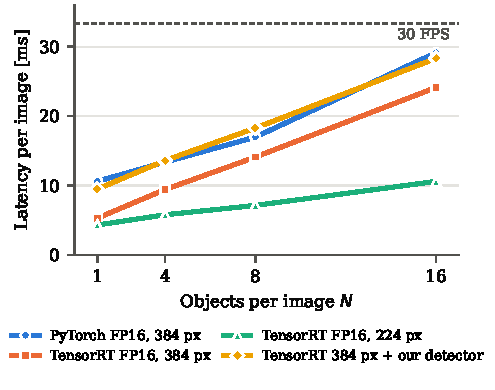
\includegraphics[width=\linewidth]{figures/latency.pdf}
  \caption{\textbf{Latency per image vs.\ number of objects} (pose pipeline from the decoded
  image to $N$ poses; LM-O model, one A100). With TensorRT FP16 and our detector, the full
  method stays above 30 FPS up to 16 objects.}
  \label{fig:latency}
\end{figure}

\paragraph{Detector.}
With the default detector (about 80\,ms per image as reported by its authors), the detector
dominates the run time and the whole method runs at about 10 FPS. Our multi-class LW-DETR
(\cref{sec:method:detector}) reaches a COCO mAP of 0.656 on the LM-O test targets, on par with
the default detections (0.657), and gives 0.654 AR with our pose model (0.645--0.650 with the
smaller ``tiny'' variant). Exporting it to TensorRT required one change: TensorRT 10.14's
\texttt{GridSample} returns wrong values for the deformable attention of LW-DETR (mAP 0.633 even
in FP32), so we implement the bilinear sampling with gather operations, which gives the same
output as PyTorch. The FP16 engine runs in 4.2\,ms per image on average (median 3.3\,ms,
including resizing, normalization and top-$k$ selection) with the same mAP (0.657), and the full
pipeline reaches 55 FPS for 8 objects at 384 px (0.654 AR), or 88 FPS at 224 px, where the
backbone costs 0.023 AR (0.643 vs.\ 0.666, two seeds each).
\todo{Jetson Orin numbers, if a device becomes available; otherwise state it as a limitation.}

\subsection{Qualitative Results}
\label{sec:exp:qualitative}
\begin{figure*}[t]
  \centering
  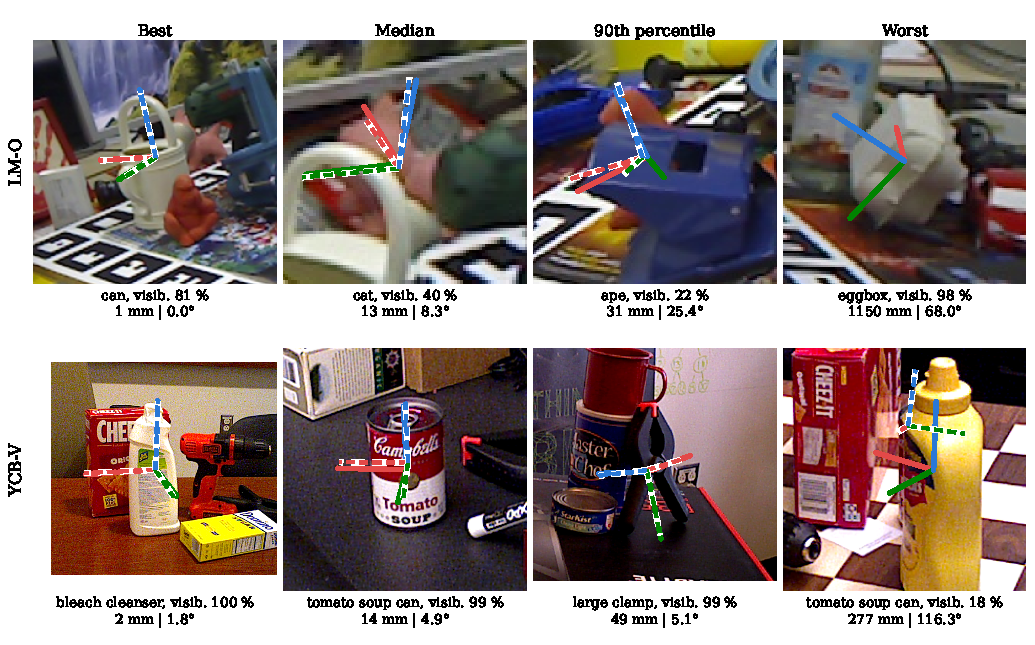
\includegraphics[width=\linewidth]{figures/qualitative.pdf}
  \caption{\textbf{Qualitative results} on LM-O (top) and YCB-V (bottom) with the default
  detections: the best, median, 90th-percentile and worst test instance, ranked by the MSSD error
  relative to the object diameter. Ground-truth axes are solid (for symmetric objects, under the
  symmetry closest to the prediction), predictions dashed; below each crop, the object, its
  visible fraction, and the translation [mm] and rotation [deg] errors. The worst LM-O case is a
  wrong detection: the predicted pose lies outside the crop.}
  \label{fig:qualitative}
\end{figure*}

\begin{figure}[t]
  \centering
  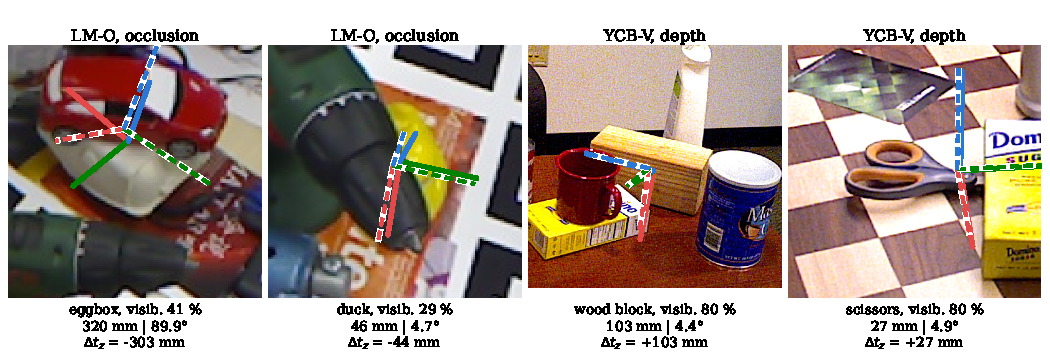
\includegraphics[width=\linewidth]{figures/failures.pdf}
  \caption{\textbf{Failure cases.} Left: heavily occluded LM-O objects (eggbox, duck), where the
  regressed depth and, for the eggbox, the rotation fail. Right: the depth bias on real YCB-V
  images; the rotation is accurate ($< 5^\circ$) but the object is estimated too far
  ($\Delta t_z > 0$).}
  \label{fig:failures}
\end{figure}

\Cref{fig:qualitative} shows typical predictions. The median errors over all test instances are
19\,mm and 4.3\textdegree{} on LM-O, and 22\,mm and 3.8\textdegree{} on YCB-V: the rotation is
usually accurate, and most of the error lies in the depth. \Cref{fig:failures} shows the two main
failure modes. First, heavily occluded objects: with less than half of the eggbox or the duck
visible, the crop contains too little of the object to regress its depth, and the eggbox, whose
appearance is ambiguous, also gets a wrong rotation. Second, a systematic depth bias on the real
YCB-V images: 89\,\% of the YCB-V instances are estimated too far (median +20\,mm), against 48\,\%
on LM-O (median $-1$\,mm). The real objects appear smaller in the images than their PBR renders
at the same depth, so a network trained on PBR images only overestimates their depth; the
weakest YCB-V objects (wood block 0.39 AR, scissors 0.41) are the most affected. Training with
the real YCB-V images should remove this bias, as it does for the methods trained on them.

\section{Conclusion}
\label{sec:conclusion}

We presented \ours{}, a multi-object extension of FastPose-ViT that regresses the 6D pose of every
object of a BOP dataset directly from its image crop, with one plain Vision Transformer and a
single linear layer shared by all objects, conditioned on the object identity by a per-object
class token. A size-invariant depth target makes the formulation independent of the camera and of
the object size, and a symmetry-aware rotation loss with translation offsets handles symmetric
objects; the apparent rotation of the original method remains the most important ingredient
(+0.11 AR). Trained on PBR images only, \ours{} reaches 0.668 AR on LM-O and 0.702 AR on YCB-V,
the best YCB-V result among PBR-only RGB methods with one model for all objects, and it loses no
accuracy in TensorRT FP16. With our own multi-class detector, the full pipeline runs at 55 FPS
for 8 objects on an A100.

Our main limitations are the depth accuracy of the directly regressed translation, which explains
most of the gap in the 3D metrics, heavily occluded objects, and a depth bias on real YCB-V
images that synthetic training data alone does not remove. Training with the real images of
YCB-V, measuring the latency on embedded hardware, and \pending{T-LESS} are the next steps.
\todo{Rewrite once T-LESS and the augmentation study are in, and once the positioning against
PViT-6D and PoseDETR is agreed.}


{\small
\IfFileExists{ieeenat_fullname.bst}{\bibliographystyle{ieeenat_fullname}}{%
  \IfFileExists{ieee_fullname.bst}{\bibliographystyle{ieee_fullname}}{\bibliographystyle{ieeetr}}}
\bibliography{references}
}

\end{document}
